\documentclass[10pt]{beamer}

\usetheme[progressbar=frametitle]{metropolis}
\usepackage{appendixnumberbeamer}

\usepackage{booktabs}
\usepackage[scale=2]{ccicons}
\usepackage{listings}
% % \usetheme[progressbar=frametitle]{metropolis}
\usepackage{appendixnumberbeamer}
\usepackage[utf8]{vietnam}
\usepackage[utf8]{inputenc}
\usepackage[vietnamese]{babel}
\usepackage[T1]{fontenc}
%\renewcommand\sfdefault{cmbr}
\usepackage{booktabs}
\usepackage[scale=2]{ccicons}
\usepackage{ragged2e}
\apptocmd{\frame}{}{\justifying}{}
\usepackage{pgfplots}
\usepgfplotslibrary{dateplot}
\usepackage[upright]{fourier}
\usepackage{tikz}



\usetikzlibrary{matrix,arrows,decorations.pathmorphing}


\definecolor{rosy}{RGB}{247, 215, 148}
\definecolor{summer}{RGB}{245, 205, 121}
\definecolor{beige}{RGB}{253, 227, 167}
\definecolor{sblack}{RGB}{64, 64, 64}
\setbeamercolor{frametitle}{bg=rosy,%bg=beige,
fg=sblack}

\usepackage{hyperref}
\hypersetup{
    colorlinks=true,
    linktoc=all,
    linkcolor=black,
}
\usepackage{relsize}
\usepackage{textpos}
\addtobeamertemplate{frametitle}{}{%
\begin{textblock*}{100mm}(\textwidth,-1.05cm)
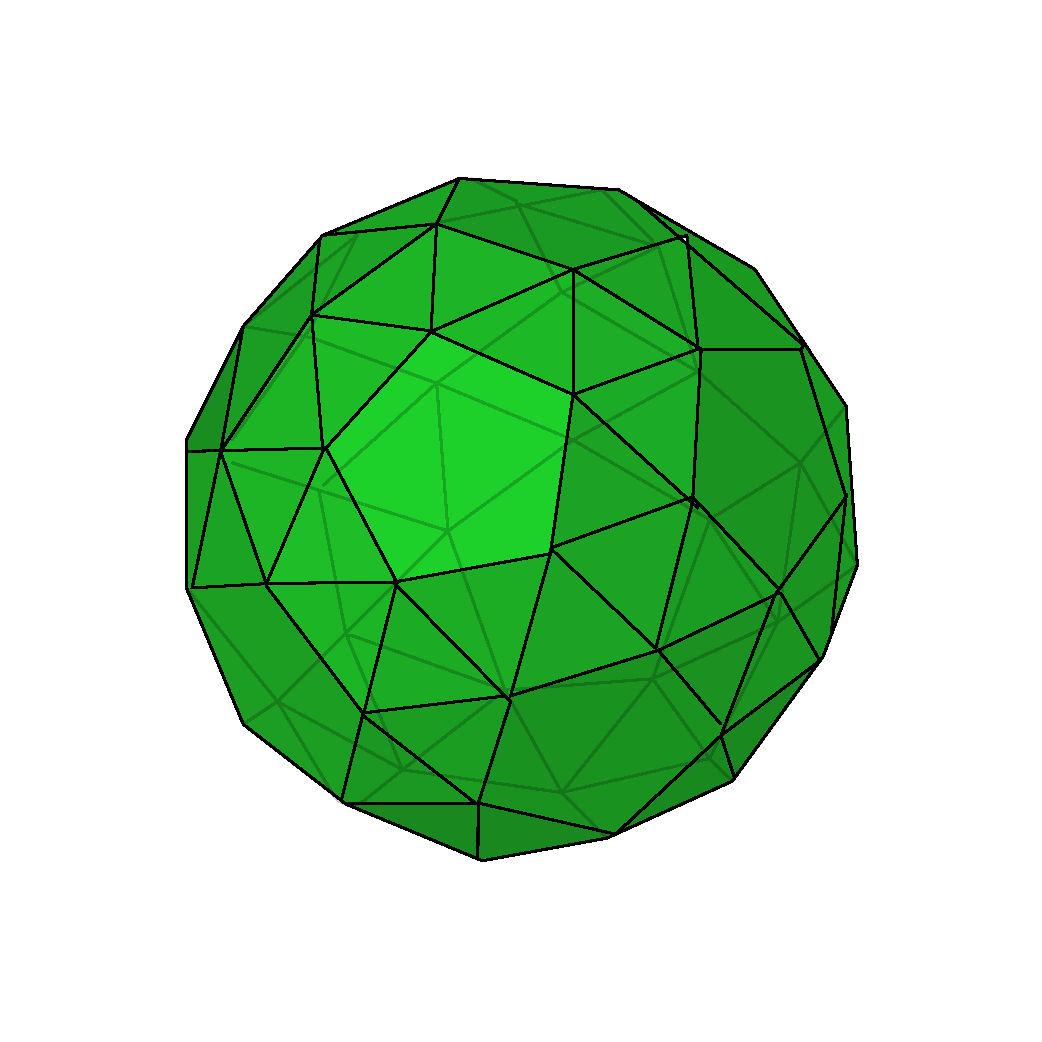
\includegraphics[height=1cm,width=1cm,keepaspectratio]{logo.pdf}
\end{textblock*}}

\usepackage{xspace}

\setbeamerfont{page number in head/foot}{size=\tiny}
\setbeamercolor{footline}{fg=gray}
\setbeamertemplate{frame footer}{PiMA 2019: The Mathematics of Deep Learning}

% \newcommand{\themename}{\textbf{\textsc{metropolis}}\xspace}
\usepackage{cmbright}

\usepackage{pgfplots}
\usepgfplotslibrary{dateplot}

\usepackage{xspace}
\newcommand{\themename}{\textbf{\textsc{metropolis}}\xspace}

\title{LẬP TRÌNH PYTHON}
\subtitle{PiMA 2019 - Python cơ bản}
\date{\today}
\date{}
\author{Phan Ngọc Tiên}
\institute{York University, Toronto, Canada}
%\titlegraphic{\hfill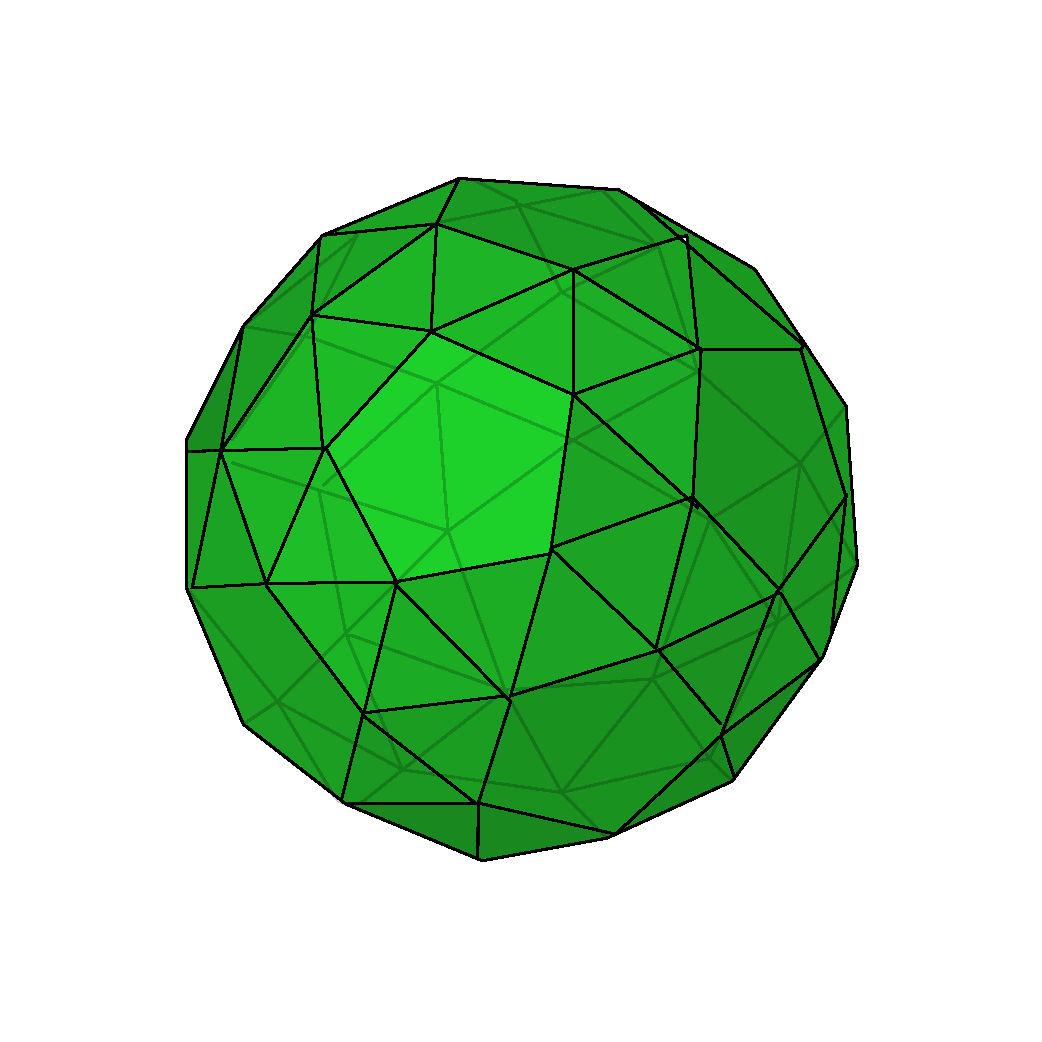
\includegraphics[height=1.5cm]{logo.pdf}}

\begin{document}

\maketitle

\begin{frame}{Mục lục}
  \setbeamertemplate{section in toc}[sections numbered]
  \tableofcontents[hideallsubsections]
\end{frame}

\section{Giới thiệu về Python}
\begin{frame}{Giới thiệu về Python}
  \begin{itemize}
    \item Python là ngôn ngữ lập trình bậc cao, ra mắt lần đầu vào năm 1991
    \item Python là ngôn ngữ lập trình đơn giản, cú pháp (syntax) đơn giản, dễ  đọc, rất gần với ngôn ngữ tự nhiên
    \item Hỗ trợ lập trình hướng cấu trúc, lập trình hướng cấu trúc và lập trình hàm (yếu)
  \end{itemize}
\end{frame}

\begin{frame}[fragile]{Basic Input/Output (Nhập xuất cơ bản)}
  \begin{verbatim}
    # Input (Nhập)
    x = input()

    # Output (Xuất)
    print(x)
  \end{verbatim}
\end{frame}

\begin{frame}[fragile]{Các phép toán}
  \begin{itemize}
    \item Python hỗ trợ các phép toán $+, -, *, /$ (chia lấy kết quả float), $//$ (chia lấy phần nguyên, kết quả int), $**$ (lên lũy thừa).

    \item Các phép biến đổi bit: $\&$ (AND), $|$ (OR), $\ \^$ (XOR).

    \item Đối với biến logic có \textbf{and, or, not}.

    \item Các phép toán so sánh $<$ (nhỏ hơn), $>$ (lớn hơn), $<=$ (nhỏ hơn hoặc bằng), $>=$ (lớn hơn hoặc bằng), $==$ (bằng)

  \end{itemize}
\end{frame}

\begin{frame}[fragile]{Các kiểu dữ liệu}
  \begin{itemize}
    \item Python tạo kiểu động (dynamically typed)
  \end{itemize}
  \begin{columns}
    \begin{column}{0.4\textwidth}
      \begin{verbatim}
        # Số nguyên (Integer)
        x = 20
        # Số thực (Float)
        y = 17.5
        # Số phức (Complex)
        z = 20 + 17j
      \end{verbatim}
    \end{column}
    \begin{column}{0.7\textwidth}
      \begin{verbatim}
        #include <iostream>
        #include <complex>
        using namespace std;

        int main() {
        int x = 20;
        double y = 17.5;
        complex<double> z4 = 1.5 + 2i;
        }
      \end{verbatim}
    \end{column}
  \end{columns}
\end{frame}

\begin{frame}[fragile]{Các kiểu dữ liệu: Boolean}
  \begin{columns}
    \begin{column}{0.4\textwidth}
      \begin{verbatim}
        # Boolean
        x = True
        y = False
      \end{verbatim}
    \end{column}
    \begin{column}{0.7\textwidth}
      \begin{verbatim}
        #include <iostream>
        #include <complex>
        using namespace std;

        int main() {
        bool x = true;
        bool y = false;
        }
      \end{verbatim}
    \end{column}
  \end{columns}
\end{frame}

\begin{frame}[fragile]{Các kiểu dữ liệu: String (Chuỗi)}
  \begin{itemize}
    \item Python
    \begin{verbatim}
      # String (Chuỗi)
      x = "PiMA 2019 'Deep Learning'"
    \end{verbatim}

    \item C++
    \begin{verbatim}
      #include <iostream>
      #include <string>
      using namespace std;

      int main() {
      string s = "PiMA 2019 'Deep Learning'";
      }
    \end{verbatim}
  \end{itemize}

\end{frame}


\begin{frame}[fragile]{Các kiểu dữ liệu: List (Danh sách)}

  \begin{itemize}
    \item Python
    \begin{verbatim}
      x = [1, 2, 3, 4, 5]
      # List can be nested (danh sách có thể lồng vào nhau)
      x = [[1, 2, 3], [4, 5, 6]]

      ## Có thể có nhiều kiểu dữ liệu trong cùng 1 danh sách
      x = [[3.14, 2], 3 + 4j, [5, 6]]
    \end{verbatim}
    \item C++
    \begin{verbatim}
      #include <iostream>
      #include <vector>
      using namespace std;
      int main() {
      int arr[] = {1, 2, 3, 4, 5, 6};
      vector <double> a {3.14, 2.71, 2.11};
      }
    \end{verbatim}
  \end{itemize}
\end{frame}

\begin{frame}[fragile]{Các kiểu dữ liệu: Dictionary (Từ Điển)}
  \begin{verbatim}
    x = {"P": "Project",
    "i": "in",
    "M": "Mathematics",
    "A": "Applications"}
  \end{verbatim}
\end{frame}

\begin{frame}[fragile]{Các kiểu dữ liệu: Tuple}
  \begin{verbatim}
    point = (1, 2, 3)

    # Lấy ra giá trị từ tuple
    x, y, z = point
  \end{verbatim}


  \only<2>{\Large Tuple vs List: điểm giống và khác nhau giữa List và Tuple là gì?}
\end{frame}


\begin{frame}[fragile]{Python cơ bản}
  Refer to notebook.
\end{frame}

\begin{frame}[fragile]{Hàm (function)}

\end{frame}

% 
% \begin{frame}[allowframebreaks]{References}
%
%   \bibliography{demo}
%   \bibliographystyle{abbrv}
%
% \end{frame}

\end{document}
